\documentclass[11pt]{article}
\usepackage[utf8]{inputenc}
\usepackage{geometry}
\geometry{a4paper, margin=0.5in}
\usepackage{tikz}
\usetikzlibrary{shapes.geometric, arrows.meta, positioning, calc, backgrounds, fit}

\title{FloodSense AI -- System Architecture Diagrams}
\author{Auto-Generated Technical Documentation}
\date{\today}

\begin{document}

\maketitle

\section*{1. High-Level Architectural Diagram}
This diagram illustrates the decoupling between the React frontend, FastAPI gateway, the autonomous Multi-Agent System (MAS), and external integrations.

\vspace{1cm}
\begin{center}
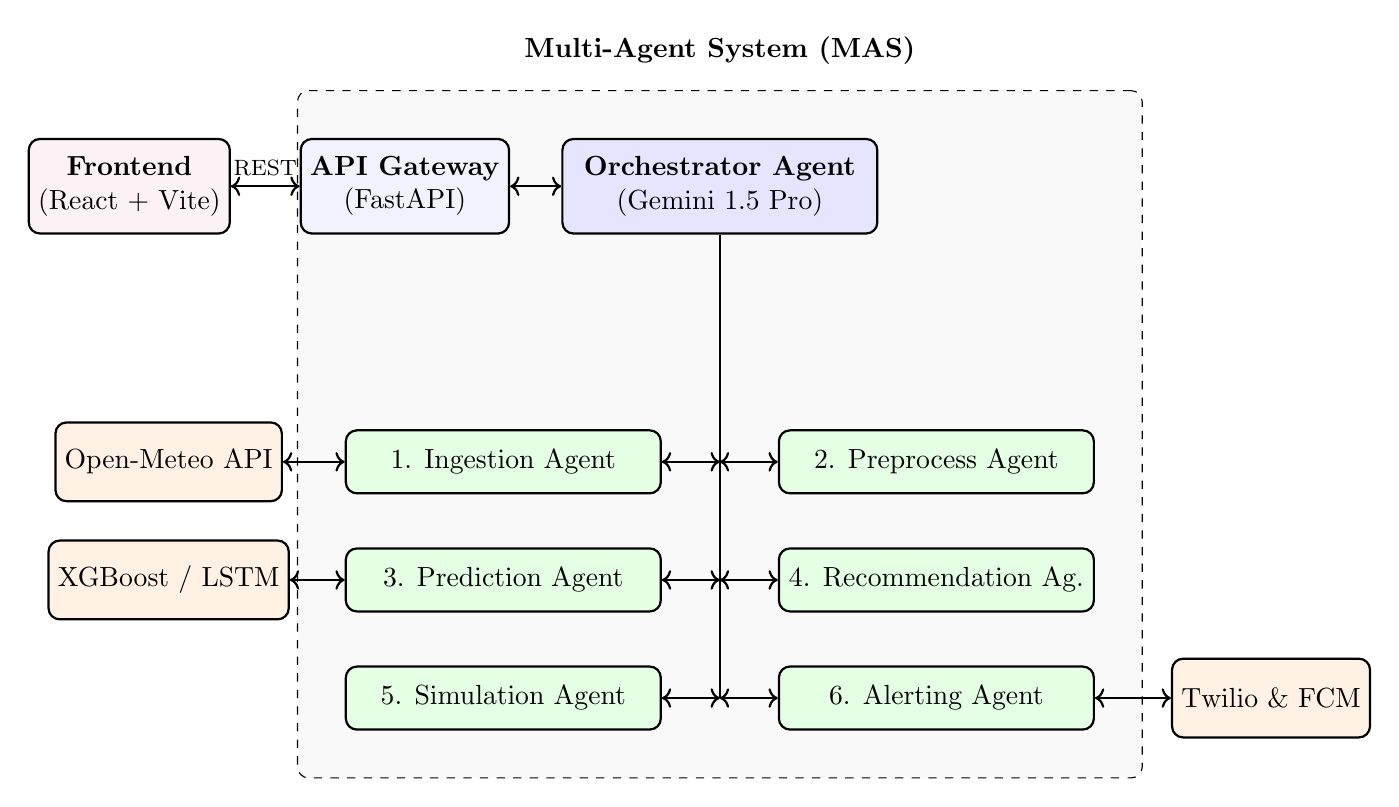
\begin{tikzpicture}[
    box/.style={rectangle, draw, rounded corners, align=center, minimum height=1.2cm, minimum width=2.5cm, fill=blue!5, thick},
    agent/.style={rectangle, draw, rounded corners, align=center, minimum height=0.8cm, minimum width=4cm, fill=green!10, thick},
    ext/.style={rectangle, draw, rounded corners, align=center, minimum height=1cm, minimum width=2.5cm, fill=orange!10, thick},
    arrow/.style={-{Stealth}, thick}
]

% Top level components
\node[box, fill=purple!5] (frontend) at (0, 0) {\textbf{Frontend} \\ (React + Vite)};
\node[box] (gateway) at (3.5, 0) {\textbf{API Gateway} \\ (FastAPI)};
\node[box, fill=blue!10, minimum width=4cm] (orchestrator) at (7.5, 0) {\textbf{Orchestrator Agent} \\ (Gemini 1.5 Pro)};

% Agents below orchestrator
\node[agent] (ingestion)    at (4.75, -3.5) {1. Ingestion Agent};
\node[agent] (preprocess)   at (10.25, -3.5) {2. Preprocess Agent};
\node[agent] (prediction)   at (4.75, -5)   {3. Prediction Agent};
\node[agent] (recommendation) at (10.25, -5) {4. Recommendation Ag.};
\node[agent] (simulation)   at (4.75, -6.5) {5. Simulation Agent};
\node[agent] (alerting)     at (10.25, -6.5) {6. Alerting Agent};

% Trunk line from Orchestrator
\draw[thick] (orchestrator.south) -- (7.5, -6.5);

% Connections from trunk to agents
\draw[arrow, <->] (7.5, -3.5) -- (ingestion.east);
\draw[arrow, <->] (7.5, -3.5) -- (preprocess.west);
\draw[arrow, <->] (7.5, -5)   -- (prediction.east);
\draw[arrow, <->] (7.5, -5)   -- (recommendation.west);
\draw[arrow, <->] (7.5, -6.5) -- (simulation.east);
\draw[arrow, <->] (7.5, -6.5) -- (alerting.west);

% MAS Background Frame
\begin{scope}[on background layer]
\node[draw, dashed, rounded corners, fit=(orchestrator)(ingestion)(preprocess)(simulation)(alerting), fill=gray!5, inner sep=0.6cm] (mas_bg) {};
\node[above=0.2cm of mas_bg.north, font=\bfseries] {Multi-Agent System (MAS)};
\end{scope}

% External APIs positioned squarely on the far sides to prevent any horizontal overlap
\node[ext] (weather)  at (0.5, -3.5) {Open-Meteo API};
\node[ext] (ml)       at (0.5, -5)   {XGBoost / LSTM};
\node[ext] (sms)      at (14.5, -6.5) {Twilio \& FCM};

% Main flow arrows
\draw[arrow, <->] (frontend) -- node[above, font=\footnotesize] {REST} (gateway);
\draw[arrow, <->] (gateway) -- (orchestrator);

% Agent to external arrows
\draw[arrow, <->] (ingestion.west) -- (weather.east);
\draw[arrow, <->] (prediction.west) -- (ml.east);
\draw[arrow, <->] (alerting.east) -- (sms.west);

\end{tikzpicture}
\end{center}

\newpage
\section*{2. Data Flow Diagram}
This diagram traces how input data (e.g., sensor readings) moves through the system, gets processed by agents, and translates into actionable recommendations and predictions.

\vspace{1cm}
\begin{center}
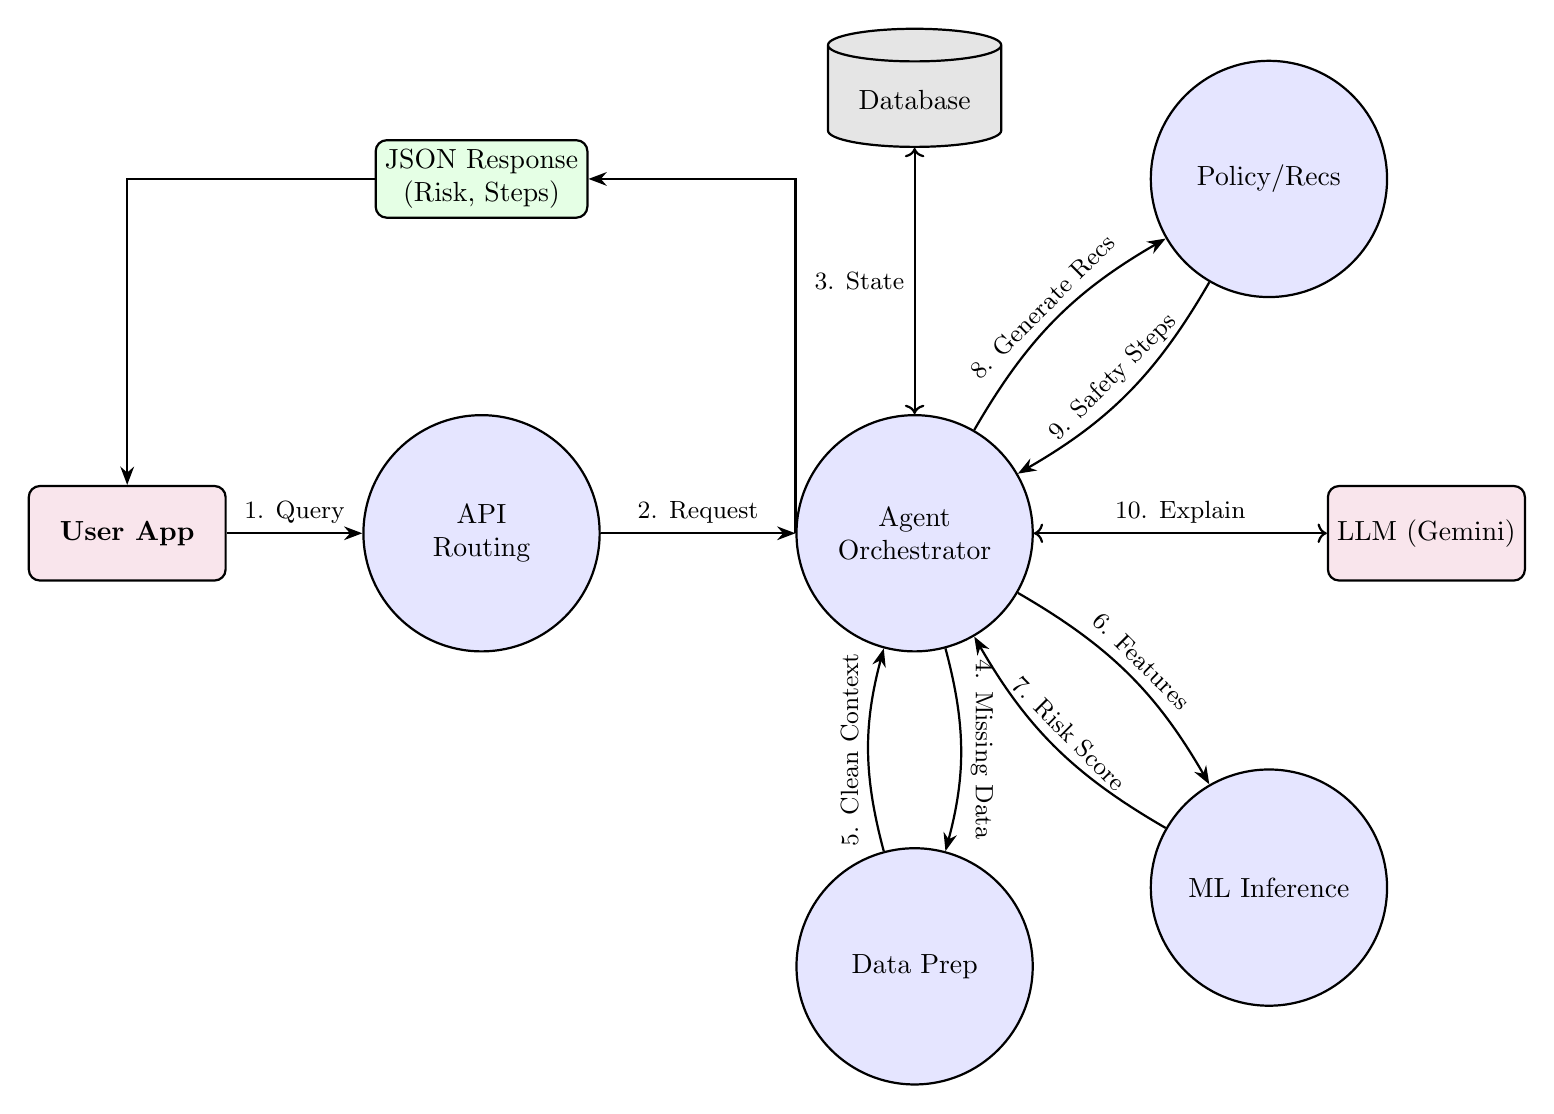
\begin{tikzpicture}[
    process/.style={circle, draw, align=center, fill=blue!10, thick, minimum width=3cm},
    data/.style={rectangle, draw, align=center, fill=green!10, thick, rounded corners},
    store/.style={cylinder, draw, shape border rotate=90, aspect=0.25, align=center, fill=gray!20, thick, minimum width=2.2cm, minimum height=1.5cm},
    ext/.style={rectangle, draw, align=center, fill=purple!10, thick, rounded corners, minimum height=1.2cm, minimum width=2.5cm},
    arrow/.style={-{Stealth}, thick}
]

\node[ext]     (user)  at (0, 0) {\textbf{User App}};
\node[process] (api)   at (4.5, 0) {API\\Routing};
\node[process] (orch)  at (10, 0) {Agent\\Orchestrator};

\node[store]   (db)    at (10,  5.5) {Database};
\node[ext]     (llm)   at (16.5, 0) {LLM (Gemini)};
\node[process] (rec)   at (14.5, 4.5) {Policy/Recs};
\node[process] (ml)    at (14.5, -4.5) {ML Inference};
\node[process] (prep)  at (10, -5.5) {Data Prep};

\node[data]    (resp)  at (4.5, 4.5) {JSON Response \\ (Risk, Steps)};

% Edges
\draw[arrow] (user) -- node[above, font=\small] {1. Query} (api);
\draw[arrow] (api) -- node[above, font=\small] {2. Request} (orch);

\draw[arrow, <->] (orch) -- node[left, font=\small] {3. State} (db);

% Use bend left=15 for all bidirectional pairs to form clean wide "eye" loops
\draw[arrow] (orch) to[bend left=15] node[sloped, above, font=\small] {4. Missing Data} (prep);
\draw[arrow] (prep) to[bend left=15] node[sloped, above, font=\small] {5. Clean Context} (orch);

\draw[arrow] (orch) to[bend left=15] node[sloped, above, font=\small] {6. Features} (ml);
\draw[arrow] (ml)   to[bend left=15] node[sloped, above, font=\small] {7. Risk Score} (orch);

\draw[arrow] (orch) to[bend left=15] node[sloped, above, font=\small] {8. Generate Recs} (rec);
\draw[arrow] (rec)  to[bend left=15] node[sloped, above, font=\small] {9. Safety Steps} (orch);

\draw[arrow, <->] (orch) -- node[above, font=\small] {10. Explain} (llm);

\draw[arrow] (orch.west) |- (resp.east);
\draw[arrow] (resp.west) -| (user.north);

\end{tikzpicture}
\end{center}

\newpage
\section*{3. User Flow Diagram}
This illustrates the end-user journey across the interactive React interface, covering the primary modules of the FloodSense application.

\vspace{1cm}
\begin{center}
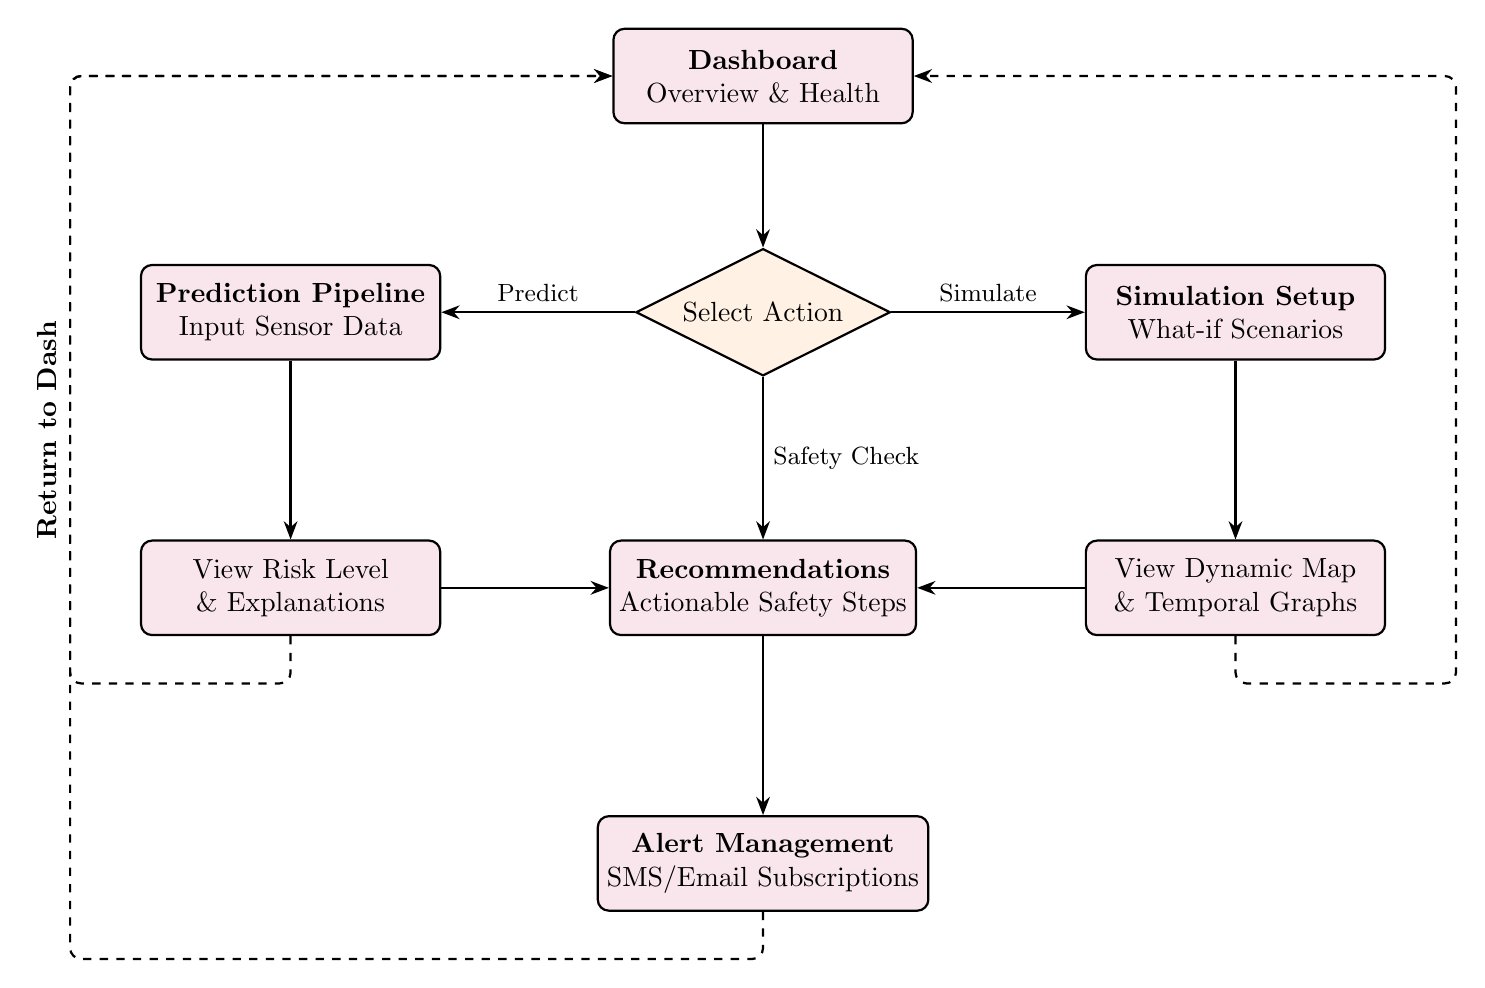
\begin{tikzpicture}[
    screen/.style={rectangle, draw, rounded corners, align=center, minimum width=3.8cm, minimum height=1.2cm, fill=purple!10, thick},
    decision/.style={diamond, draw, align=center, fill=orange!10, thick, aspect=2, minimum width=2.5cm},
    arrow/.style={-{Stealth}, thick}
]

\node[screen]   (landing)   at (6, 0)   {\textbf{Dashboard} \\ Overview \& Health};
\node[decision] (choice)    at (6, -3) {Select Action};

\node[screen]   (predict)   at (0, -3) {\textbf{Prediction Pipeline} \\ Input Sensor Data};
\node[screen]   (pred_view) at (0, -6.5) {View Risk Level \\ \& Explanations};

\node[screen]   (sim)       at (12, -3) {\textbf{Simulation Setup} \\ What-if Scenarios};
\node[screen]   (sim_view)  at (12, -6.5) {View Dynamic Map \\ \& Temporal Graphs};

\node[screen]   (recs)      at (6, -6.5) {\textbf{Recommendations} \\ Actionable Safety Steps};
\node[screen]   (alerts)    at (6, -10) {\textbf{Alert Management} \\ SMS/Email Subscriptions};

% Edges
\draw[arrow] (landing) -- (choice);

\draw[arrow] (choice) -- node[above, font=\small] {Predict} (predict);
\draw[arrow] (predict) -- (pred_view);
\draw[arrow] (pred_view) -- (recs);

\draw[arrow] (choice) -- node[above, font=\small] {Simulate} (sim);
\draw[arrow] (sim) -- (sim_view);
\draw[arrow] (sim_view) -- (recs);

\draw[arrow] (choice) -- node[right, font=\small] {Safety Check} (recs);

\draw[arrow] (recs) -- (alerts);

% Return Paths using clean far-margins to prevent crossing nodes
\draw[arrow, dashed, rounded corners] (pred_view.south) -- ++(0, -0.6) -| (-2.8, 0) -- (landing.west);
\draw[arrow, dashed, rounded corners] (sim_view.south)  -- ++(0, -0.6) -| (14.8, 0) -- (landing.east);
\draw[arrow, dashed, rounded corners] (alerts.south)    -- ++(0, -0.6) -| (-2.8, 0) -- (landing.west);

\node[font=\bfseries, rotate=90] at (-3.1, -4.5) {Return to Dash};

\end{tikzpicture}
\end{center}

\end{document}
